\section{Implementacja}

\subsection{Zmaterializowana lista agregatów}
\subsubsection{Pojęcie agregatu}

Na potrzeby projektu zostało zdefiniowane pojęcie agregatu jako obiektu który zawiera jednostkę informacji skojarzoną z danym kluczem. Inaczej mówiąc, jednostka informacji jest rozumiana jako zgrupowana wartość według klucza.

Rozpatrujemy listę zmaterializowanych agregatów dla przestrzennego klucza temporalno-czasowego, których kluczem jest identyfikator miejsca (\emph{venueId}) oraz znacznik czasowy (\emph{timestamp}) wyrównany do okna czasowego (np minuty, godziny, dnia, miesiąca, roku)\footnote{Poprzez wyrównanie stempla czasowego do godziny mamy na myśli stempel czasowy pierwszej sekundy danej godziny, dla roku pierwszą sekundę pierszego dnia itd.}.

Zostały zdefiniowane następujące struktury w języku Java:

\begin{itemize}[noitemsep]
  \item \emph{IAggregateKey} - klucz agregatu, obiekt immutable (klucz może być złożony),
  \item \emph{IAggregateValue} - wartość agregatu, obiekt immutable (wartość agregatu może składać się z wielu pól),
  \item \emph{Aggregate} - zmaterializowany agregat, obiekt immutable (połączenie klucza z wartością).
\end{itemize}

\lstinputlisting[language=java]{../MaterializedAggregationFramework/src/pl/polsl/tpdia/mal/IAggregateKey.java}

\lstinputlisting[language=java]{../MaterializedAggregationFramework/src/pl/polsl/tpdia/mal/IAggregateValue.java}

\lstinputlisting[language=java]{../MaterializedAggregationFramework/src/pl/polsl/tpdia/mal/Aggregate.java}

\subsection{Mapowanie danych na agregaty}

Każda porcja informacji (krotka) napływająca strumieniowo, która trafia do systemu ma ściśle okrśloną strukturę, tj. klucz oraz zestaw wartości. Jednocześnie każda krotka sama w sobie jest agregatem (wartością atomową). Zdefiniowane zostały interfejsy pozwalające mapować agregaty na inne agregaty nazywane Mapperami (\emph{IAggregateMapper}).

Mappery przekształcają agregat w agregat o tych samych wartościach, lecz o zmienionym kluczu. Intencją jest zmmieniona granulacja klucza agregatu, na przykład implementacją mapera może być przekształcenie klucza krotki na wyrównany co do miesiąca, aby produkotwać krotki o wartościach pogrupowanych po miesiącu.

\lstinputlisting[language=java]{../MaterializedAggregationFramework/src/pl/polsl/tpdia/mal/IAggregateKey.java}

\subsection{Mappery oraz struktura agregatów}

Mapery mogą zostać połączone w łańcuch (\emph{Mapper Chain}), tak, aby dana krotka została zamapowana na wszystkie możliwe (w zależności od kontekstu, w jakim został zbudowany łańcuch) granulacje. Przykładowo istnieje możliwość połączenia Mapperów w łańcuch tak, aby wartość atomowa została przekształcona na agregat minutowy, następnie agregat minutowy na godzinowy, następnie agregat godzinowy na dniowy, itd. Produkowanie agregatów w łańcuchu prezentuje schemat \ref{fig:impl-mapping-chain}

\begin{figure}[h!]
  \centering
    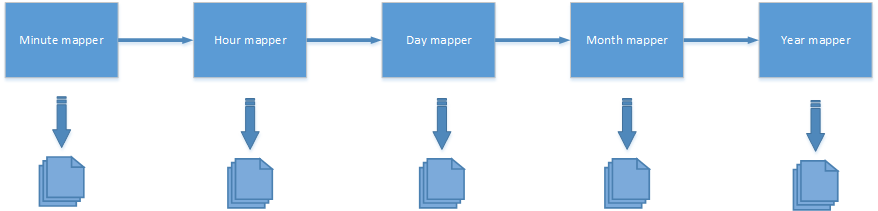
\includegraphics[scale=0.75]{impl-mapping-chain.png}
  \caption{Zasada łączenia Mapperów w łańcuch}
  \label{fig:impl-mapping-chain}
\end{figure}

Agregaty logicznie ułożone są w kompozycję przypominającą dynamicznie tworzoną strukturę drzewiastą wg klucza. Fizycznie nie ma między nimi żadnych powiązań (referencji), a źródło danych, w którym utrwalane są agregaty, może być odpytywane punktowo.

\subsection{Tworzenie agregatów i procesor zapytań}

Każda porcja informacji, kótra trafia do systemu, zamieniana jest na agregat i iterpretowana jako wartość atomowa. Operacja ta ma na celu narzucenie struktury porcji informacji, czyli klucza oraz zestawu wartości. W ten sposób tworzone są pierwsze agregaty.

Zapytania zadane systemowi są przekazywane \emph{Procesorowi zapytań}, który rozbijane je na XX fazy:

\begin{itemize}[noitemsep]
  \item analiza semantyczna zapytania,
  \item na podstawie łańcucha maperów zaplanowanie wszystkich możliwie największych agregatów, z których można złożyć odpowiedź
  \item kaskadowe zbieranie wyników ze wszystkich istniejących agregatów oraz (jeżeli nie istnieją) tworzenie nowych, wcześniej zaplanowanych agregatów, z wyników pośrednich,
  \item złączenie wyników z możliwie największych agregatów i udzielenie odpowiedzi
\end{itemize}

Agregaty mogą być tworzone w dowolnych momentach, a w szczególności:

\begin{itemize}[noitemsep]
  \item w momencie pojawienia się krotki w systemie\footnote{Podobnie jak struktury indeksujace w bazach daych} lub,
  \item przy pierwszym zapytaniu lub,
  \item w zależności od charakterystyki i obciążenia systemu (np jest więcej zapisów, niż odczytów), obliczanie agregatów może zostać opóźniane
\end{itemize}

\subsubsection{Sposób wyznaczania tworzenia agregatów przez procesor zapytań}

Gdy do systemu trafia zapytanie zakresowe po kluczu \emph{IAggregateKey} o wyliczenie wartości bazjąych na \emph{IAggregateValue} procesor zapytań analizuje zakres zapytania i na podstawie łańcucha mapperów przygotowuje listę wszystkich możliwie największych agregatów, które mogą zostać wykorzystane do zwrócenia wyniku zapytania.

\textbf{Przyład}

Przyjmujemy założenie, że agregacja informacji następuje po miejsach (\emph{venueId}) oraz po dacie wyrównanej do: roku, miesiąca, dnia, godziny, minuty. Jeżeli zostaje zadane zapytanie zakresowe od 2014-09-24 do 2014-11-05, wyznaczane są następujące możliwie największe agregaty:

\begin{itemize}[noitemsep]
  \item dzienne od 2014-09-24 do 2014-09-30,
  \item miesięczne od 2014-10-01 do 2014-10-31,
  \item dzienne od 2014-11-01 do 2014-11-05,
\end{itemize}

\subsubsection{Drążenie danych - wyznaczanie nieistniejących agregatów}

Jeżeli agregaty, o które system został zapytany jeszcze nie istnieją w trwałym źródle danych, dekomponowane są na możliwie największe podagregaty (\emph{drążenie danych}). Jeżeli któreś podagregaty są już wcześniej obliczone, nie ma potrzeby ich ponownej dekompozycji, natomiast dla podagregatów, które nie są policzone proces powtarza się, aż proces dekompozycji sięgnie danych źródłowych, które są agregatami atomowymi.

Schemat działania zobrazowany jest na rysunku \ref{impl-aggregate-chunking}.

\begin{figure}[h!]
  \centering
    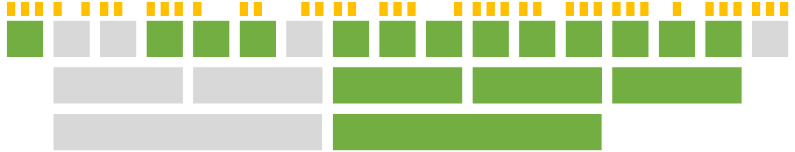
\includegraphics[scale=0.75]{impl-aggregate-chunking.png}
  \caption{Dekomponowanie agregatów oraz drążenie danych. Zielone kwadraty oznaczają obliczone pola, białe nieistniejące, żółtym kolorem oznaczone zostały agregaty atomowe, czyli dane źródłowe}
  \label{fig:impl-aggregate-chunking}
\end{figure}

Agregaty tworzone są poprzez zagregow

\subsection{Aktualizowanie agregatów}

Od dołu do góry.

\emph{Rule 3: Handle Stream Imperfections (Delayed, Missing and Out-of-Order Data)} \cite{stream-processing-streamsql}

Powyższe struktury moga zostać odzworowane jako encje bazodanowe za pomocą biblioteki umożliwiającej mapowanie obiektowo-relacyjne, na przykład za pomocą Hibernate. Z uwagi na fakt, iż przedstawiana jest jedynie koncepcja rozwiązania, zgodnie z ideą tworzenia architektury heksagonalnej (nie pożenionej z żadnym konkretnym frameworkiem), struktry pozostawnioe zostały jako zwykłe klasy Java.
